
%(BEGIN_QUESTION)
% Copyright 2006, Tony R. Kuphaldt, released under the Creative Commons Attribution License (v 1.0)
% This means you may do almost anything with this work of mine, so long as you give me proper credit

En vanlig malefeil i instrumenter kalles {\it hysterese}.  En veldig lignende type malefeil kalles {\it dodbånd}.  Beskriv hva disse feilene er, og skill mellom dem.

\underbar{file i00091}
%(END_QUESTION)





%(BEGIN_ANSWER)

Hysterese og dodbånd er ikke nøyaktig samme type kalibreringsfeil, men de er naert beslektet.  ``Dodbånd'' refererer til et omrade av instrumentmalingen ved reversering av inngang der utgangen ikke endrer seg i det hele tatt.  Et vanlig eksempel er et ``slarkete'' styresystem i en bil, der rattet ma dreies mye for a ta opp ``slark'' (mekanisk slakk) i styringen.

Hysterese refererer til situasjonen der en reversering av inngangen gir en umiddelbar, men ikke proporsjonal, reversering av utgangen.  Dette sees ofte i luftdrevne ventiler, der lufttrykk virker mot en stor fjær for a posisjonere ventilen nøyaktig.  Ideelt sett vil ventilen bevege seg proporsjonalt med lufttrykkssignalet, og denne posisjoneringen vil vaere bade repeterbar og nøyaktig.  Dessverre gir friksjon i ventilen hysterese: et annet lufttrykk kan vaere nodvendig for a posisjonere ventilen til samme aapning nar den apner versus nar den lukker, men i motsetning til dodbånd vil {\it enhver} reversering av signal (retning: okende vs. minkende) fa ventilen til a bevege seg litt.

Sammenlign de følgende overforingsfunksjonsgrafene for a forsta forskjellen mellom hysterese og dodbånd:

$$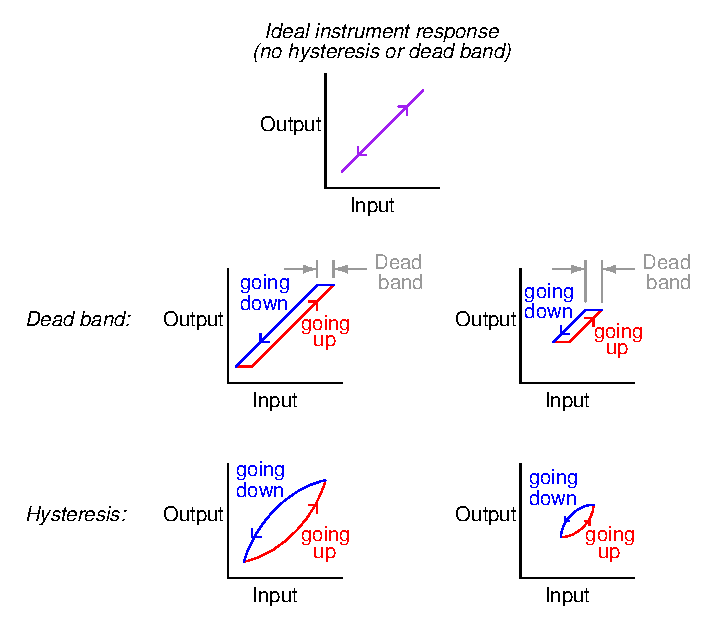
\includegraphics[width=15.5cm]{i00091x01.eps}$$

Bade dodbånd og hysterese er typisk mekaniske fenomener.  Elektroniske kretser viser sjelden slike ``artefakter'' av maling eller regulering.  Dodbånd og hysterese forekommer oftere sammen enn hver for seg i et instrument.

Interessant nok er begge effektene til stede i magnetiske kretser.  Magnetiseringskurvene for typisk transformatorkjernestål og jern er klassiske eksempler pa hysterese, mens magnetiseringskurven for ferritt (i metningsomradet) ligger ganske naer det som er en ren representasjon av dodbånd.

%(END_ANSWER)





%(BEGIN_NOTES)


%INDEX% Calibration, deadband: definition
%INDEX% Calibration, hysteresis: definition

%(END_NOTES)


